% CVPR 2022 Paper Template
% based on the CVPR template provided by Ming-Ming Cheng (https://github.com/MCG-NKU/CVPR_Template)
% modified and extended by Stefan Roth (stefan.roth@NOSPAMtu-darmstadt.de)

\documentclass[10pt,twocolumn,letterpaper]{article}

%%%%%%%%% PAPER TYPE  - PLEASE UPDATE FOR FINAL VERSION
%\usepackage[review]{cvpr}      % To produce the REVIEW version
%\usepackage{cvpr}              % To produce the CAMERA-READY version
\usepackage[pagenumbers]{cvpr} % To force page numbers, e.g. for an arXiv version

% Include other packages here, before hyperref.
\usepackage{graphicx}
\usepackage{amsmath}
\usepackage{amssymb}
\usepackage{pifont}
\usepackage{booktabs}
\usepackage{multirow}
\usepackage{url}

\newcommand{\aca}[1]{{\color{red}#1}}

% It is strongly recommended to use hyperref, especially for the review version.
% hyperref with option pagebackref eases the reviewers' job.
% Please disable hyperref *only* if you encounter grave issues, e.g. with the
% file validation for the camera-ready version.
%
% If you comment hyperref and then uncomment it, you should delete
% ReviewTempalte.aux before re-running LaTeX.
% (Or just hit 'q' on the first LaTeX run, let it finish, and you
%  should be clear).
\usepackage[pagebackref,breaklinks,colorlinks]{hyperref}


% Support for easy cross-referencing
\usepackage[capitalize]{cleveref}
\crefname{section}{Sec.}{Secs.}
\Crefname{section}{Section}{Sections}
\Crefname{table}{Table}{Tables}
\crefname{table}{Tab.}{Tabs.}


%%%%%%%%% PAPER ID  - PLEASE UPDATE
\def\cvprPaperID{*****} % *** Enter the CVPR Paper ID here
\def\confName{CVPR}
\def\confYear{2022}


\begin{document}

%%%%%%%%% TITLE - PLEASE UPDATE
\title{Attck Monocular Depth Estimation Model with a Sticker}

% \author{First Author\\
% Institution1\\
% Institution1 address\\
% {\tt\small firstauthor@i1.org}
% % For a paper whose authors are all at the same institution,
% % omit the following lines up until the closing ``}''.
% % Additional authors and addresses can be added with ``\and'',
% % just like the second author.
% % To save space, use either the email address or home page, not both
% \and
% Second Author\\
% Institution2\\
% First line of institution2 address\\
% {\tt\small secondauthor@i2.org}
% }
\author{Meng Pan, Fangjun Huang$^\dagger$\\
 School of Computer Science and Engineering, 
Sun Yat-sen University, China\\
{\tt\small panm9@mail2.sysu.edu.cn, huangfj@mail.sysu.edu.cn
}}
\maketitle
\def\thefootnote{$\dagger$}\footnotetext{
	Corresponding author}\def\thefootnote{\arabic{footnote}}

%%%%%%%%% ABSTRACT
\begin{abstract}
	DNNs have been demonstrated that their performance 
	can be degraded by imperceptible perturbations. 
	Monocular Depth Estimation networks with 
	DNNs likewise encounter such a dilemma. 
	This attack diagram, adding perturbations, 
	is not implementable and capturable for a sensor, 
	which means it is an ideal attack diagram. 
	An implementable and applicable attack diagram in 
	the physical world is needed. To this end, we 
	address this by sticking patches into indoor scenes. 
	We proposed an automatic searching and 
	transformation method. In the searching phase, 
	the patch is dispatched to an appropriate and 
	sensitive location exploiting the MDE's gradient. 
	In the transformation phase, the patch alternates 
	its appearance according to its location. 
	In doing this, we can generate destructive, 
	inconspicuous adversarial examples. 
	This whole process doesn't rely on any generate
	networks, which makes it fast and light.
	We evaluate our method on NYU depth v2, 
	experiments show that our method 
	eliminates 6\% of RMSE in 0.8s 
	meanwhile 
	keeping remarkable inconspicuousness.
\end{abstract}

\section{Introduction}
With the rapid development of 
Deep Neural Networks(DNNs), many excellent 
Monocular Depth Estimation~(MDE) methods 
base on DNNs have been proposed recently. 
However, according to Szegedy's 
research~\cite{Szegedy_2014_ICLR}, DNNs are 
prone to be attacked by adversarial examples: 
when an imperceptible 
small perturbation is added to an input image, the classifier 
based on DNNs will classify the obtained image, knowned as
adversarial examples, into a wrong category with high probability. 
Adversarial examples have been found not only on classification tasks 
but also on logical regression tasks, such as 
semantic segmentation and 
object recognition. MDE also fail to get rid of this dilemma.
As learned perception models are increasingly
deployed on autonomous driving vehicles, 
researchers attach more and more attention to
attacking MDE models.
%mistaking a stop sign for a speed limit or causing
%obstacles to disappear can cause immense damage.
%So as a kind of 3D scene perception solution, MDE 
%algorithms need to be 
%robust and reliable.

The threat of adverserial example on MDE algorithms was 
first studied by Wong~\textit{et al}~\cite{Wong_2020_NIPS}. 
They conducted 
comprehensive and rigorous experiments to explore the impact 
of pixel attacks on MDE, including attacking the whole 
depth map of a scene, attacking the depth map of one 
single object in the scene, and even making a specific 
object vanished completely on the depth map by 
adding perturbations. 

\begin{figure}
	\hspace{-0.5cm}
	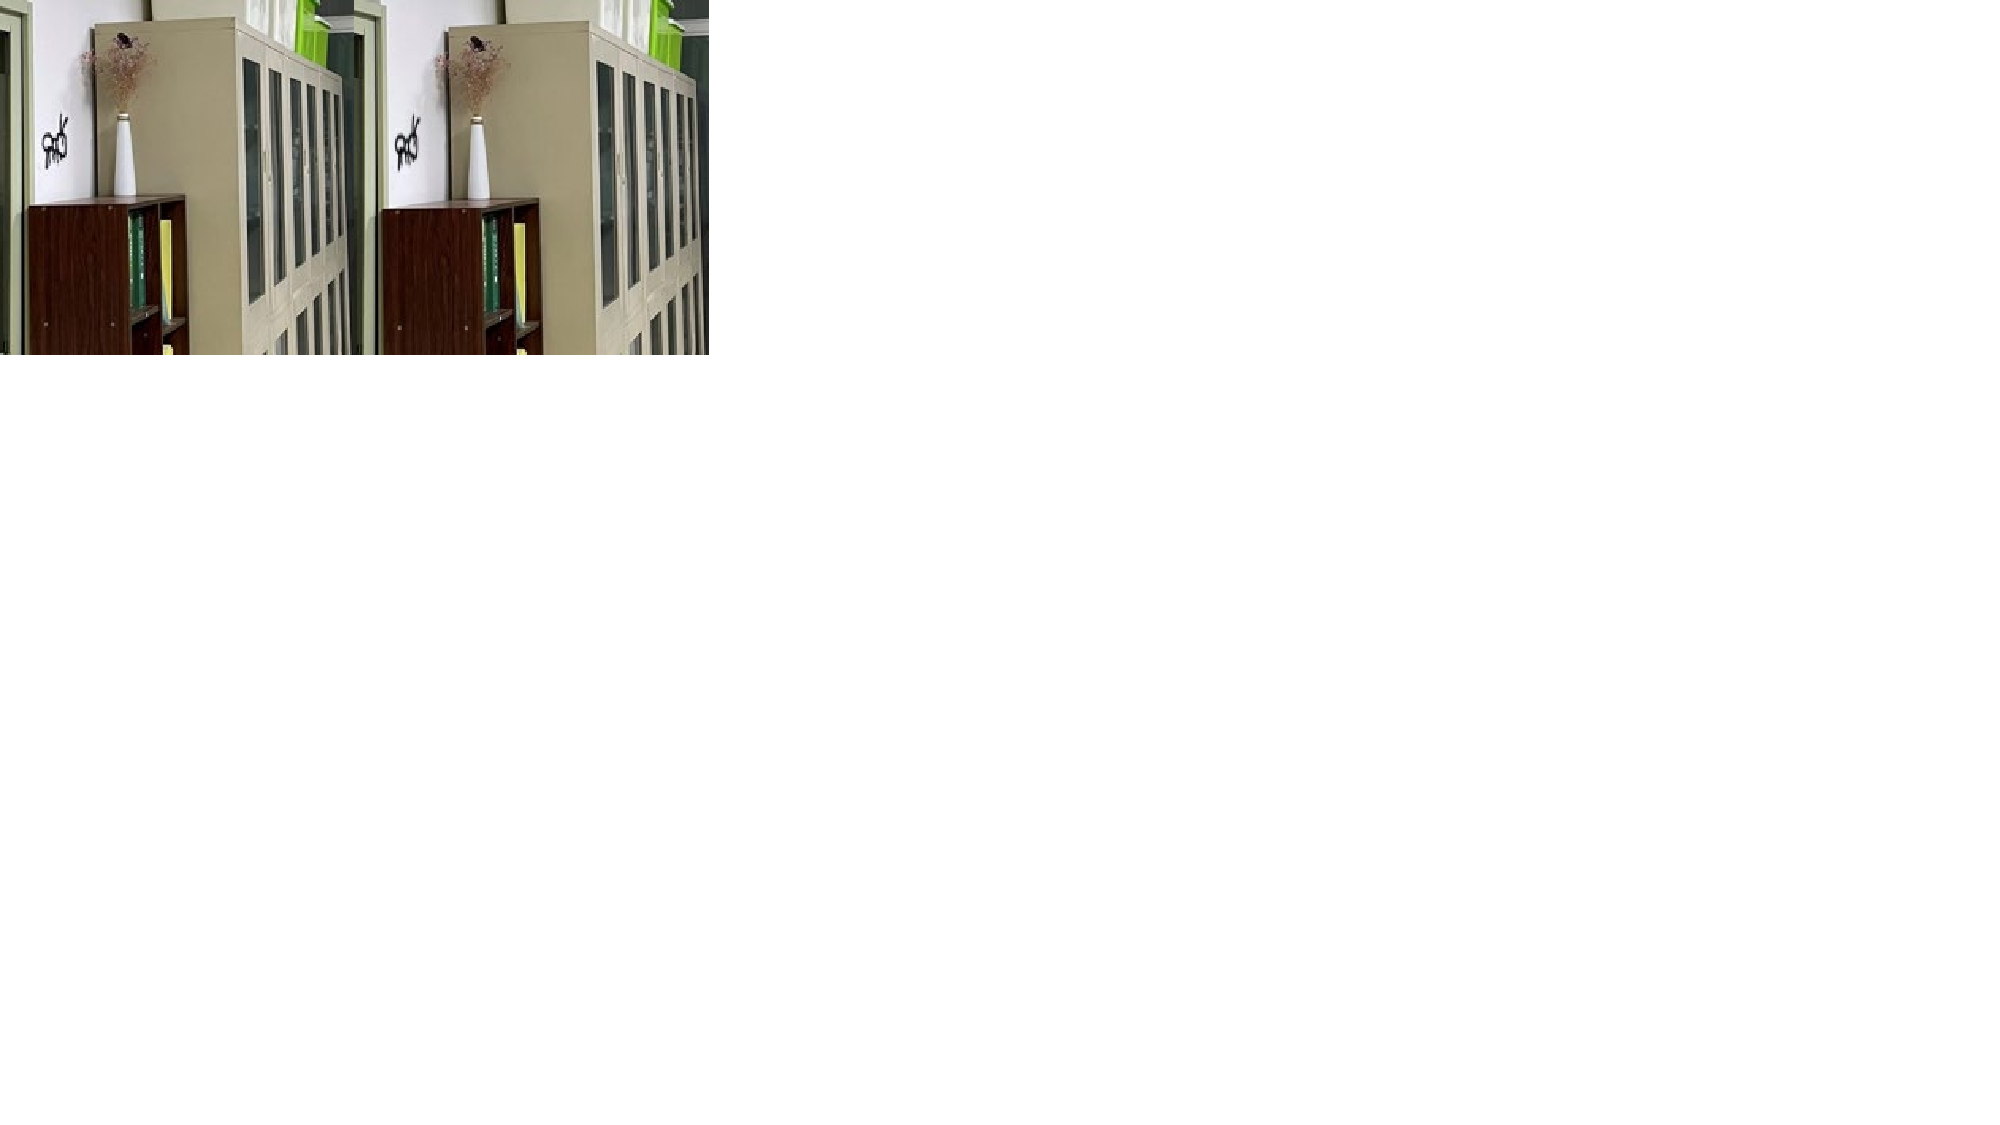
\includegraphics[width=0.5\textwidth]{imgs/preview.pdf}
	\caption{Preview of our patch attack method. 
	The adversarial example generated in pixel leveal
	by our concealed attack method(a). 
	We stick a printed drawing in the physical world~(b), and
	Note that this was shot in our office, 
	not the dataset scene we used in the experiment part.
	}
	\label[]{effect}
\end{figure}
Although the research of Wong~\textit{et al} is pioneering and 
enlightening on attacking a MDE model,
but their method is hard to be realized
in the physical world, because
the perturbations added on the benign images can not 
be captured by a camera. 

However, it is feasible to attack DNNs by adversarial 
examples generated with visible patches in the physical world.
Many works have emerged to explore this attack paradigm recently. 
Brown et al.~\cite{Brown_2017_arxiv} 
abandon the camouflage of the attack, 
and they attack DNNs by sticking an apparent, randomly transformed 
patch on benign images, which is optimized cross-scenes to raise the 
probability that it is misclassified as the target category.
In doing so, they obtained a robust and universal patch.
Nevertheless, the adversary's attack intention will expose 
easily as a result of 
the unnatural, conspicuous patches. 

Thus, researchers begin to 
pay attention to the concealment of adversarial examples.
Sharif et al.~\cite{Sharif_2017_CCS} tack the concealment 
problem by disguising the patches as accessories. 
Specifically, they attacked a face recognition 
system by wearing an artificial glasses frame,
the pattern of which is optimized by gradient 
descent with the goal of misrecognition. 
In doing so, they are misrecognized by the victim face recognition
system with the printed glasses frame.

Similarly, for better concealment, 
Hu~\textit{et al}~\cite{Hu_2021_ICCV} disguise tha patches as
the pattern on shirts to attack human detection models. 
They first detect all humans in the benign image and pin   
optimizable patches generated through a GAN on the body areas 
to obtain adversarial
examples. 
Kong et al.~\cite{Kong_2020_CVPR} also use a GAN to generate 
patches.
howerver, instead of generating directly, their patches are 
generated by adding perturbations through the GAN.
%Concretely, they collect advertisement posters and send them
%into a GAN to generate adversarial examples by 
%adding perturbations. Finally the perturbated patches are
%artificially stuck to street billboards, which is inconspicuousness
%for posters. 
%This method achieves better inconspicuousness, yet 
%the process of sticking the patch to billboards is labor consuming.

The locations of the patches are fixed in 
\cite{Sharif_2017_CCS, Hu_2021_ICCV,Kong_2020_CVPR}, 
conceivably, the locations of patches also have an impact 
on the attack success rate. 
Eykholt et al.~\cite{Eykholt_2018_CVPR} demonstrate this 
hypothesis through empirical experiments and they locate this 
area by visualizing the perturbations added using 
$L_1$ regularization. 
Instead of locating the vulnerable areas by visualizing 
the perturbations, 
they locate the vulnerable areas by a attention model, 
which takes the 
benign image as input, outputs a mask that indicates where 
is more vulnerable. 

Indeed, affiliated GAN and attention networks enhance 
the concealment of the adversary, 
but the time and space complexity also have been increased.
In this paper, we take physical realizability and 
inconspicuousness into accout, and design a fast and automatic
method to attack MDE algorithms.
Fig.~\ref{effect}(a) shows the outline of our method.
After searching for the optimal location through gradient 
descent, we alter the patch's appearance according to the 
visual effect and 'stick' it to the optimal location In
pixel level to generate our adversarial examples.
Meanwhile, in Fig.~\ref{effect}(b), we print the patch
and stick it in the physical world.
It can be seen that adversarial example in digital world 
and physical world can not be distiguished.
This indicate that our adversarial examples generated
on pixel level can be simulated through sticking a printed patch 
on the real scene.

The contributions of this work are as follows:
\begin{itemize}
	\item We are the first to apply patch attack on MDE
	tasks.
	\item  A fast, automatic, inconspicuous attack 
	method is proposed. In this method, a learnable 
	matrix is designed to update the patch's location
	based on attack effect and visual quality using gradient 
	descent. 
	\item We apply perspective transform according to visual 
	effect to alter the patch's appearance and make 
	it looks inconspicuous. 
	\item Experiments show that our method generate destructive 
	while concealed adversarial examples.
\end{itemize}.

The structure in the rest paper is organized as
follows. After a review of MDE and patch attacks in
Sec.~\ref{Background}, we introduce our method 
concretely in Sec.~\ref{Method}. Then we visualize 
the effect of our location searching phase and attack a
MDE network in Sec.~\ref{Experiments}. Finally We
analyze our patch attack method in Sec.~\ref{Conclusion}.

\section{Background}
\label[]{Background}
In this paper, we concentrate on patch attack on MDE models. 
Therefore, we will give a brief introduction for MDE task. 
%Note that we are the first to attack MDE model with patches,
%the related works only involved image classification,
%traffic sign recognition, face recognition, etc. 

\begin{figure}[hb]
	\centering
	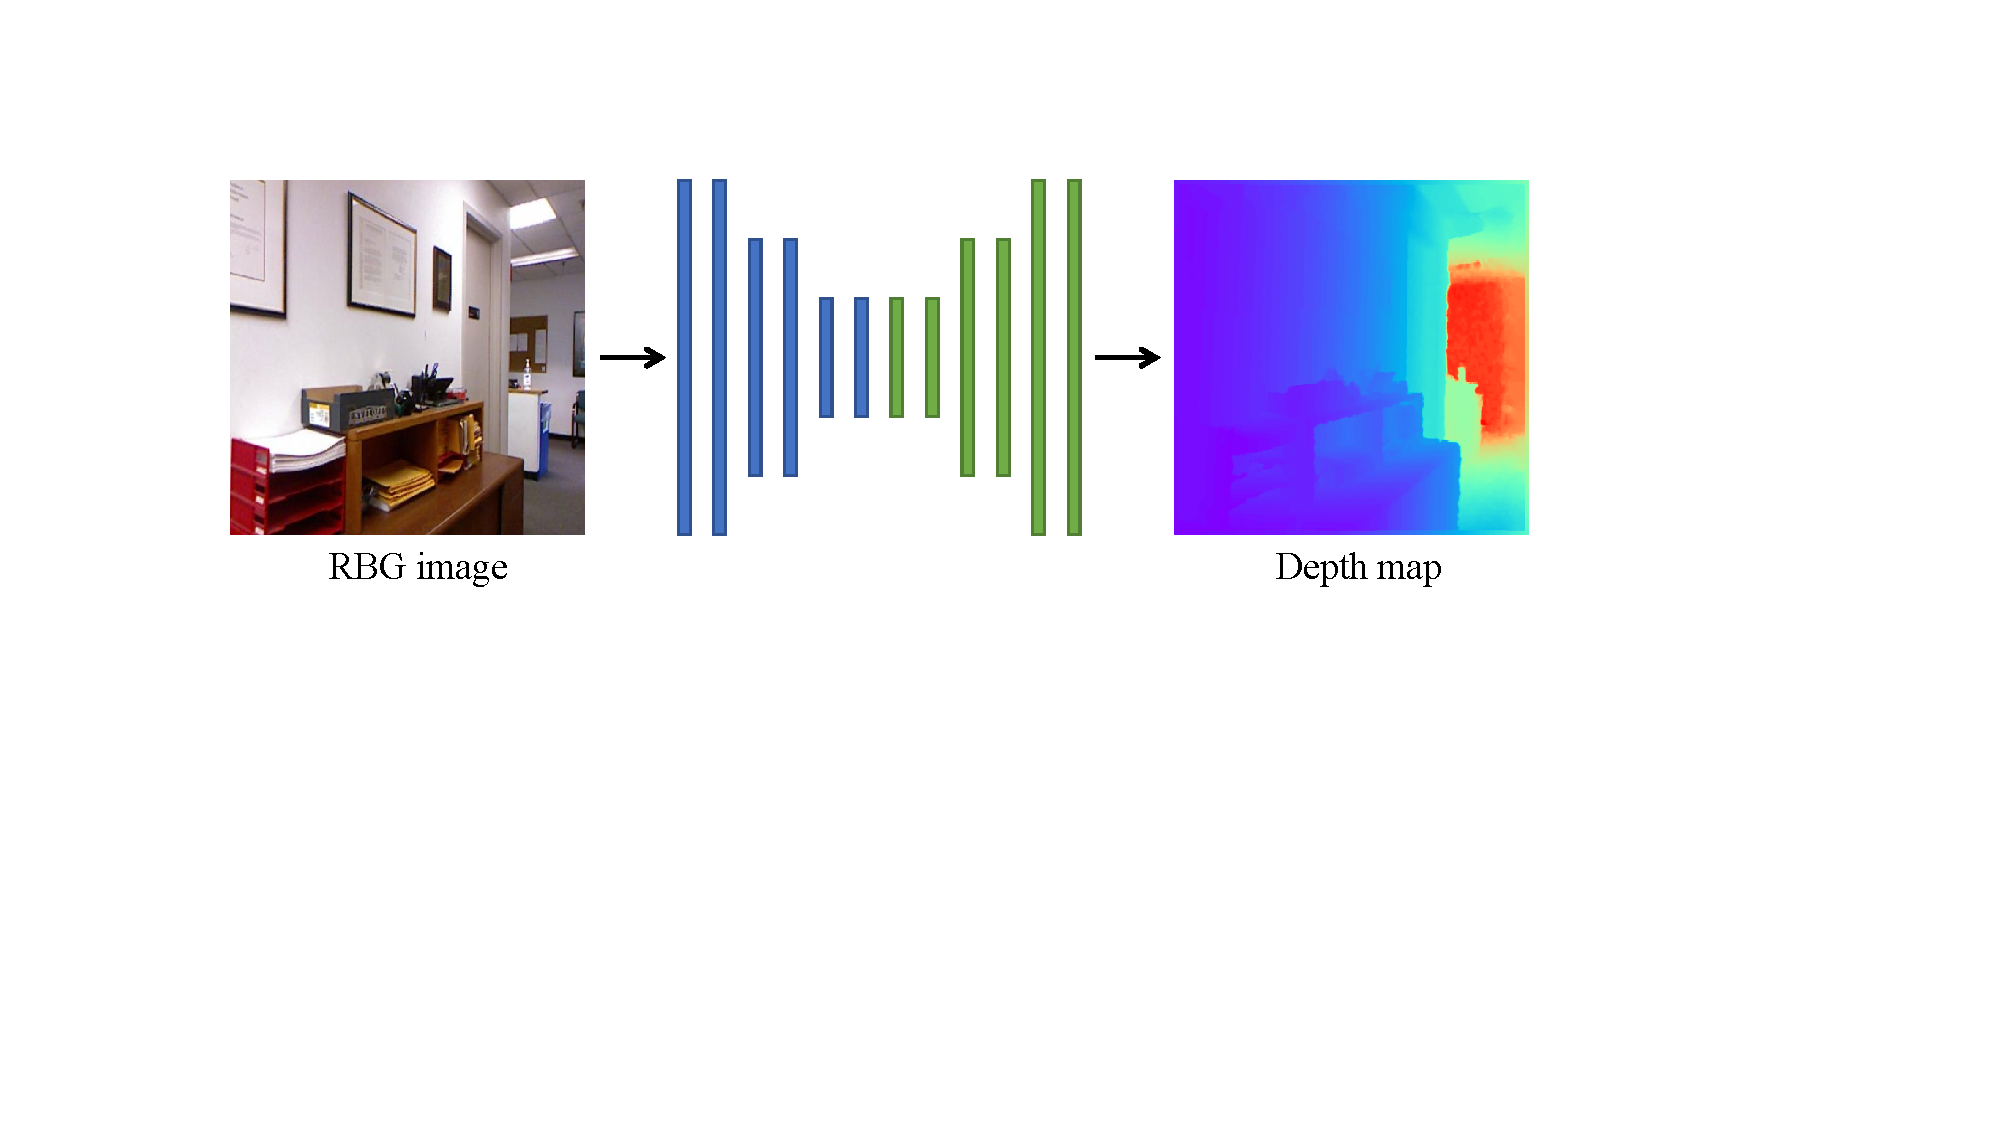
\includegraphics[width=1\linewidth]{imgs/MDE.pdf}
	\caption{A common stream of MDE algorithms in inference stage.}
	\label[]{stream of mde}
\end{figure}
With the rapid development of DNNs, MDE task achieves
satisfactory progress. 
The problem of predicting
a depth map from a single RGB image can be treated as
a supervised learning problem.
Denote the space of RGB images as $\mathcal{I}$ and 
the domain of ground 
truth depth maps as $\mathcal{D}$, given a training set 
$\mathbb{T}={(I^{H \times W \times 3}, D^{* H \times W})}$, 
$I \in \mathcal{I}$ and $D^* \in \mathcal{D}$, 
a MDE model $f_{mde}$ can learn a non-linear mapping
$f_{mde}: \mathcal{I} \rightarrow \mathcal{D^*}$
by optimizing the objective function: 
\begin{align}
	\min \Vert f_{mde}(I^{adv}) - D^{*} \Vert
\end{align}
where $|| \cdot ||$ denotes a metric for distance.
Fig.~\ref{stream of mde} shows a common inference stream of a 
MDE model:
A RGB image is fed into the trained MDE model, which generate a dense 
depth map from the RGB image. 

In this paper, we use Fastdepth~\cite{Wofk_2019_ICRA},
an efficient and lightweight encoder-decoder MDE network,
as the victim model to study the effect of our adversarial examples. 
%\subsubsection{Supervised}
%DNNs learn through the supervision of ground truth labels 
%annotated artificially. Since the mapping from a single image 
%to a depth map is very complicated, this supervised learning 
%manner is very suitable for MDE tasks. The initial work adopts 
%this \textbf{intuitive endoder-decoder} concept. 
%Eigen et al.~\cite{Eigen_2014_nips} designed two hierarchical 
%neural networks to predict 
%the depth map in coarse and fine respectively.
%A network was proposed subsequently by them~\cite{Eigen_2015_ICCV}, 
%in which three 
%different tasks, depth estimation, segmentation and 
%normals prediction was integrated into one model.
%Lee~\cite{lee_2019_arxiv} coined novel local planar 
%guidance layers and locate 
%them at different scale decoding phases. 
%As a result of this, final fine depth maps are densely 
%restored from small to big.
%Some researches~\cite{Li_2018_ACCV,cao_2017_CSVT,Fu_2018_CVPR} 
%address this problem by formulizing it as 
%a \textbf{classification} problem. 
%Discrete depth labels are prepared by separating 
%continuous depth value, which are then used to supervise 
%the training process.
%While using \textbf{relative depth information} to predict depth 
%indirectly is also a effective solution.
%Lee~\cite{Lee_2019_CVPR} proposed a method to predict depth from 
%relative depth. 
%They first estimate relative depth by utilizing rank-1 property, 
%then the final depth maps are reconstructed through these relative 
%depth maps.

%\subsubsection{Unsupervised}
%Although there exist some datasets with ground truth depth 
%annotation, dense and accurate depth maps are labor-consuming and rare. 
%In that case, unsupervised methods dominate recently.
%Godard et al.~\cite{Godard_2017_CVPR} exploit the left-right 
%consistency of binocular image pairs
%to tackle this issue: 
%with a decently predicted disparity, 
%the two images sampled from a binocular camera can 
%synthesize each other. 
%A consecutive vedio sequence can provide a constrain for MDE.
%Given a middle frame and its former, later frame sampled from a video, 
%DNNs can estimate the camera pose and the depth, with which we can 
%restore the other two frames. Based on this constrain, camera pose 
%and depth can be learned jointly~\cite{Zhou_2017_CVPR}.
%However, there is a flaw in both video and binocular solutions.
%On the one hand, binocular image pairs methods struggle in occlusion 
%and texture-copy problems, yet, on the other hand, as an 
%alternative method, 
%predicting depth from a video performs unsatisfactorily 
%when it comes to relatively stationary objects.
%To address this, Godard et al.~\cite{Godard_2019_ICCV} 
%proposed a multi-scale reconstruction
%loss and a automasking approach to ignore relatively stationary objects.

\begin{figure*}[htb]
	\centering
	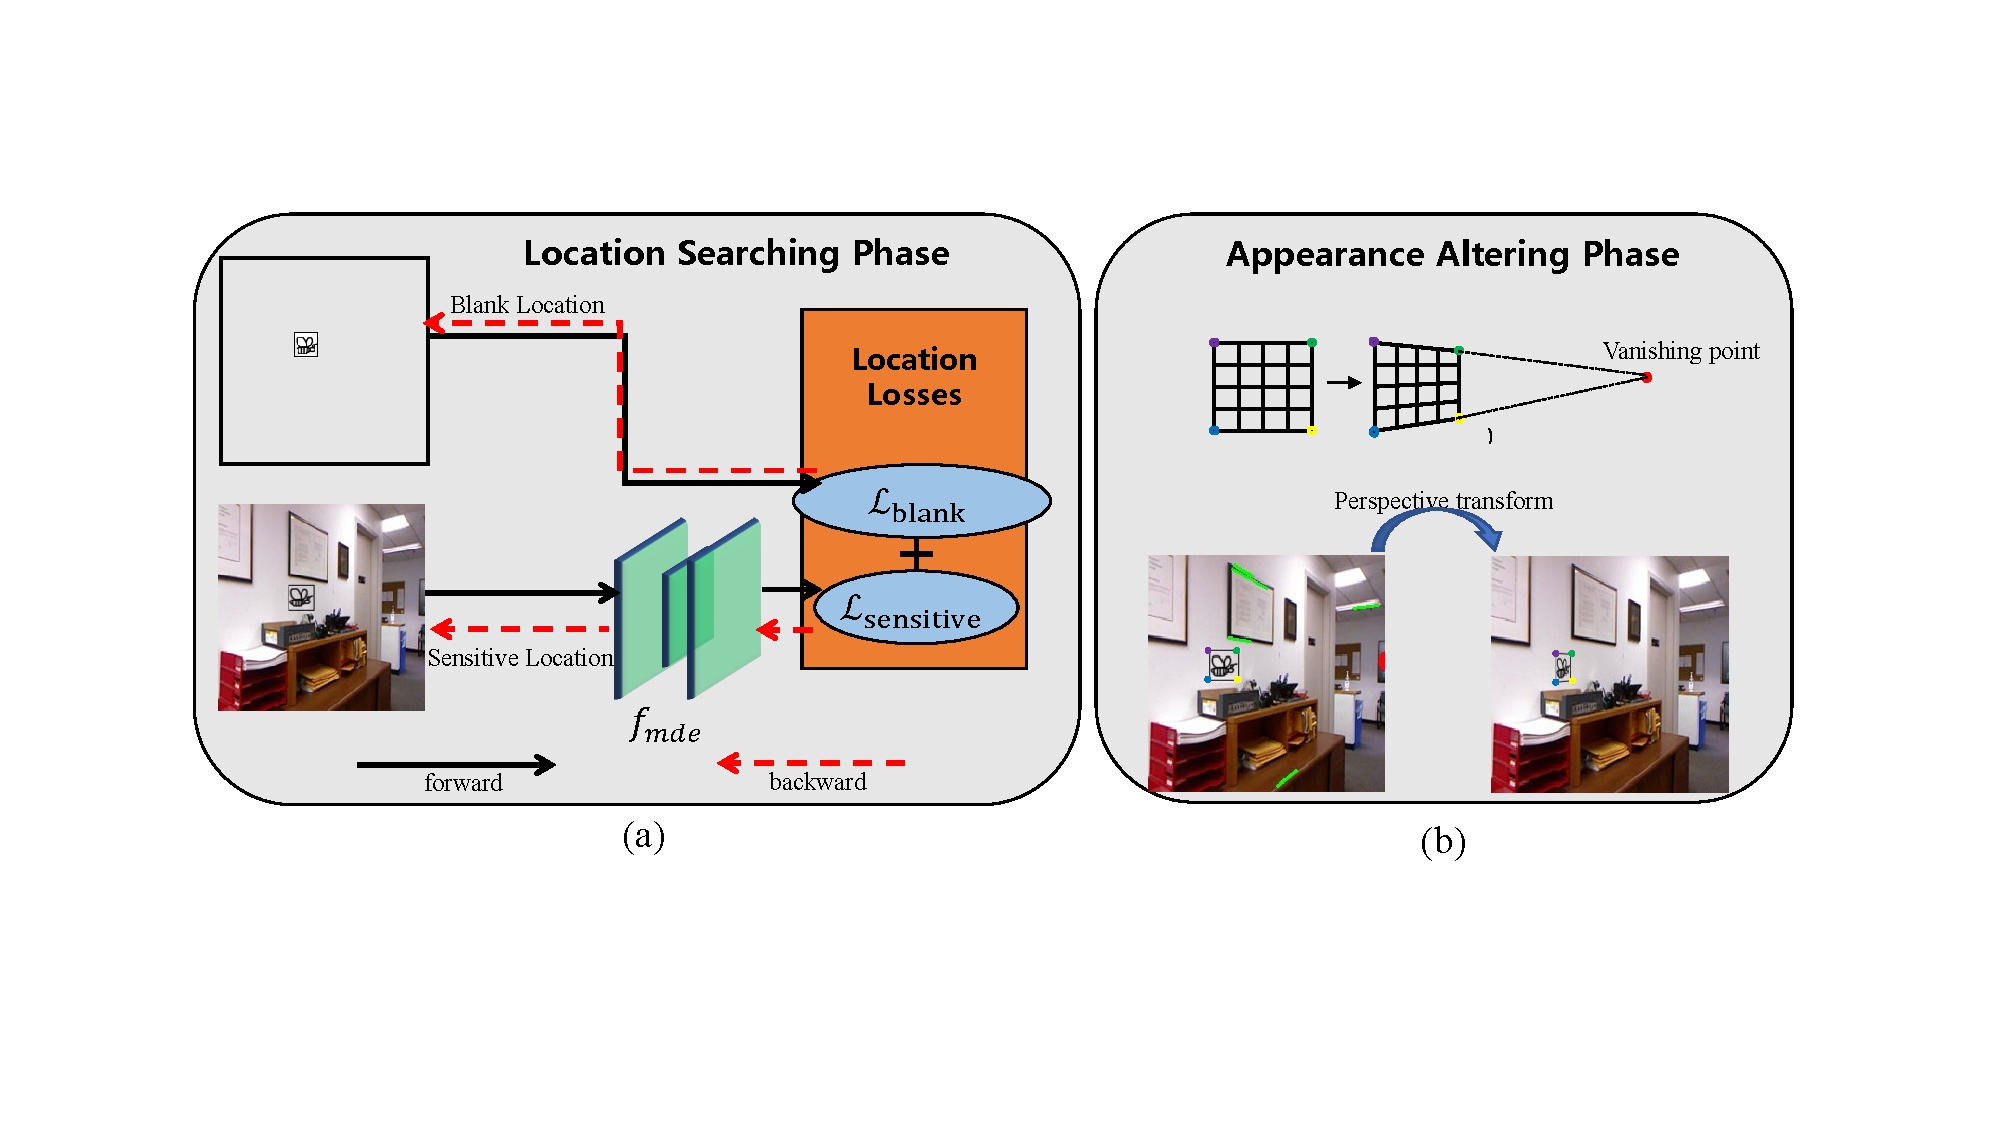
\includegraphics[width=1\textwidth]{imgs/stream.pdf}
	\caption{Stream of our MDE attacking method. 
	The whole stream consists of two phases: (a) location
	searching phase and (b) altering appearance phase. They
	are described concretely in Sec.~\ref{Location Searching}
	and Sec.~\ref{Appearance Altering}, respectively.}
	\label[]{stream}
\end{figure*}
\section{Method}
\label[]{Method}
To obtain adversarial examples with a patch,
there are two problems to be tackled: the patch's location 
and the patch's appearance.
Therefore, we design a two-phase method, 
which is shown in Fig.~\ref{stream}.
The first phase named \textbf{Location Searching Phase} 
searches for a vulnerable and inconspicuousness 
location on the benign image and the second
named \textbf{Appearance Altering Phase} 
alters the patch's appearance to make it inconspicuous.

Then the location searching phase and appearance altering 
phase are presented in Sec.~\ref{Location Searching} 
and Sec.~\ref{Appearance Altering}, respectively.

\subsection{Location Searching}
\label[]{Location Searching}
In this subsection, we will describe our location searching 
phase in detail, of which consists patch design, objective function,
and optimization of the location.
The location searching phase can be seen in 
Fig~\ref{stream}(a). 
%Current works leverage a GAN to add perturbations on patterns or 
%generate patterns, which has more time and spatial complexity. 
%In this section, we will introduce our fast and light optimal 
%method in detail, which searches the most destructive area and 
%transforms the patches to a more rational style before sticking.

\subsubsection{Patch Design}
\label[]{Patch Design}
\begin{figure}[b]
	\centering
	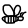
\includegraphics[width=0.1\textwidth]{imgs/patch.png}
	\caption{Our patch selected from QuickDraw. 
	We put the patch in a black box for better visualization.}
	\label[]{patch}
\end{figure}
Considering that elaborately designed 
perturbations can hardly be captured by consumer cameras, 
we propose to obtain adversarial examples $I^{adv}$ 
by sticking visible patches $\delta^{h\times w}$ to benign images $I$.

For better inconspicuousness, 
we disguise the patch a graffiti, 
which still not shows attack intention when it is noticed in a scene.
Therefore, we select a simple line-drawn drawing 
from QuickDraw~\cite{quickdraw},
a collection of 50 million hand-writing drawings across 345 categories,
as our patch. The drawing is shown in Fig.~\ref{patch},
with which our adversarial examples are defined as follows:
\begin{align}
	I^{adv} = (1-m) \odot I + m \odot \delta
	\label[]{traditional_definition}
\end{align}
where $m$ is a mask $m:\{0,1\}^{H \times W}$ that covers
the patch area with 1 and others with 0,
$\odot$ is element-wise multiplication.  
\begin{figure}[b]
	\centering
	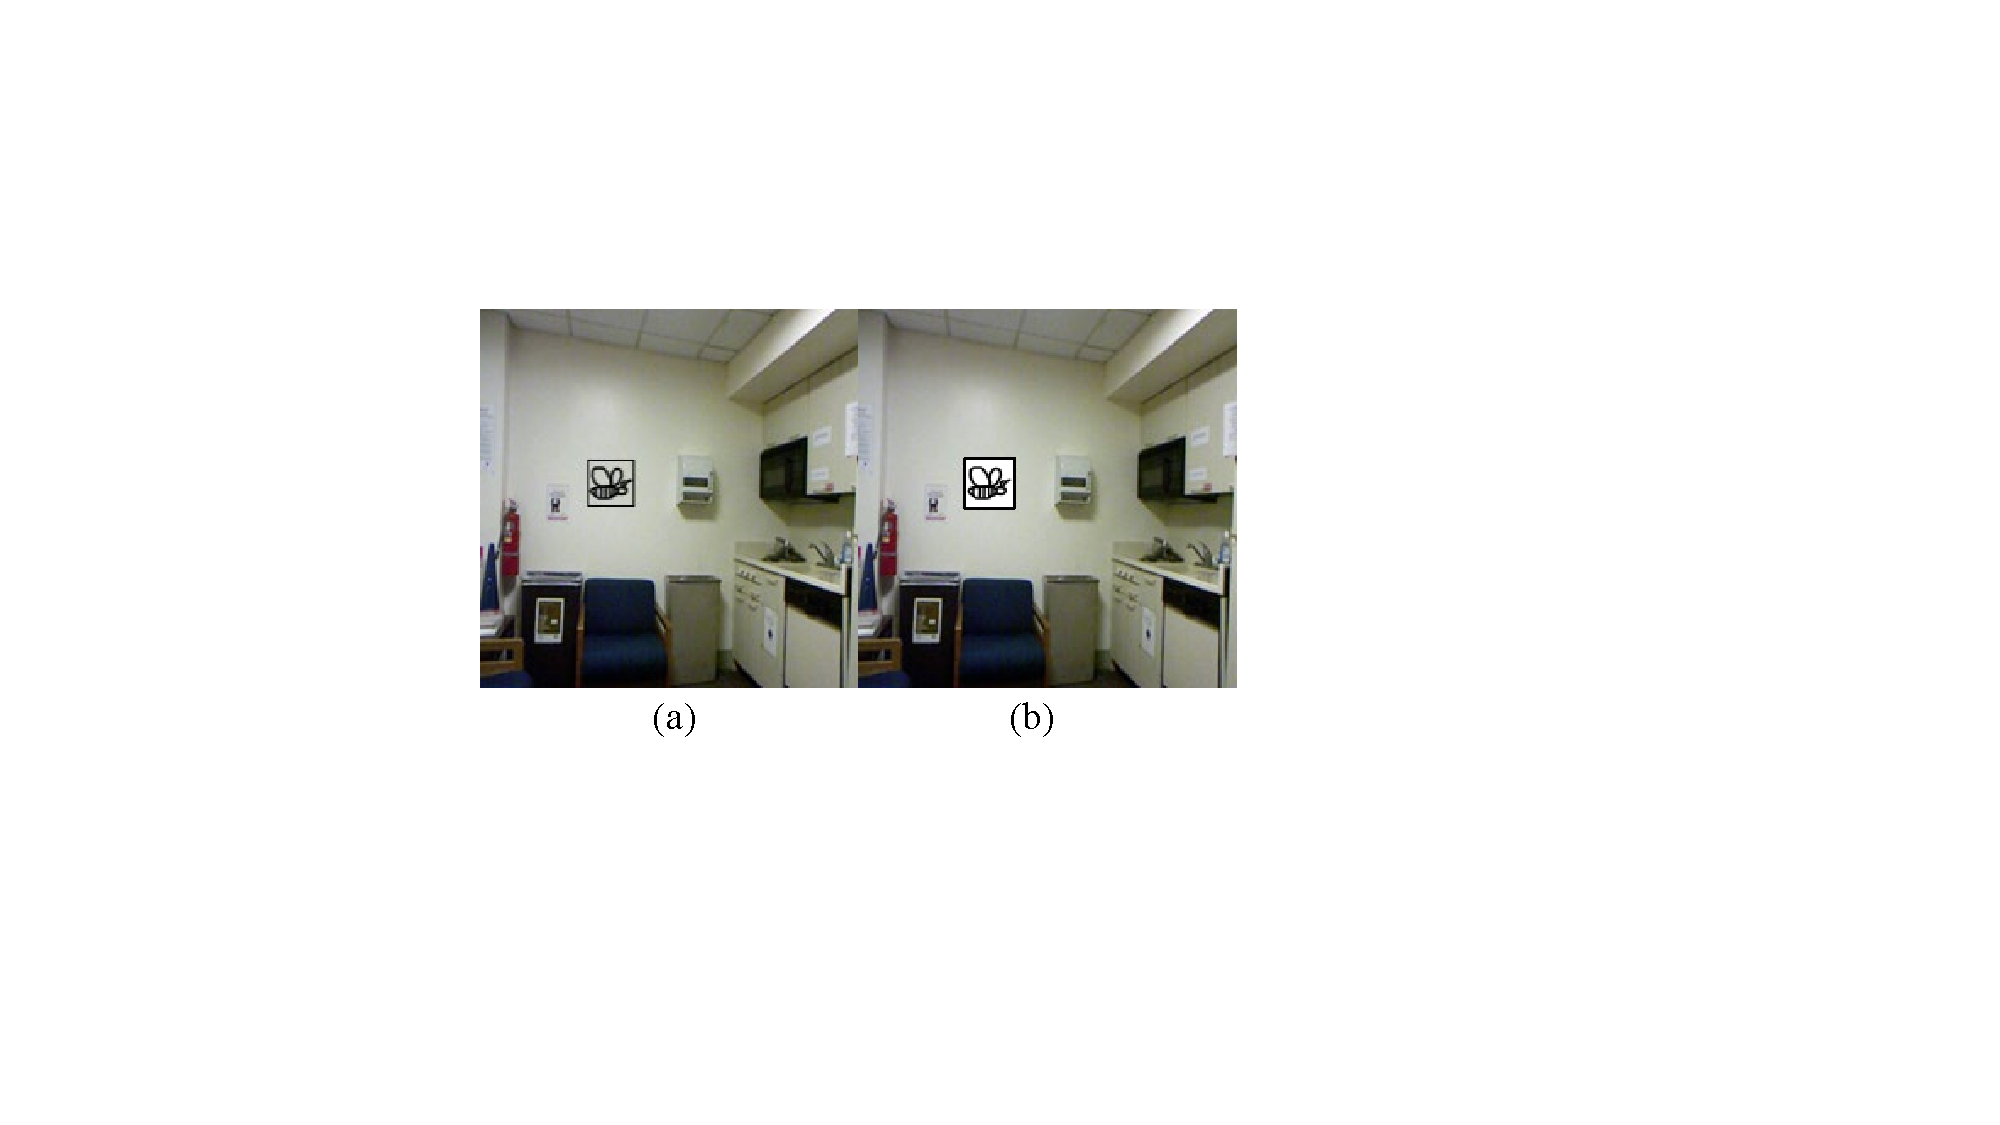
\includegraphics[width=0.45\textwidth]{imgs/definitions.pdf}
	\caption{Two definition of the adversarial examples. 
	(a) is the traditional definition used in prior works.
	(b) is our definition, 
	which reduces the modification to $I$ and makes
	the patch looks like a graffiti.}
	\label[]{diff_definition}
\end{figure}
We extend $\delta$ to size of $H \times W$ by padding 1
around it to conduct the element-wise multiplication.
The definition of Eq.~\ref{traditional_definition} modifies
the whole patch area,
to reduce modifications to $I$, 
our final definition of $I^{adv}$ is:
\begin{align}
	I^{adv} = I - I \odot \delta
	\label[]{our_definition}
\end{align}

Instead adding perturbations on a patch
or generating a patch, we select a patch and put it on a specific
location of the benign
image to generate destructive and concealed adversarial examples. 
Exhaustively searching on $I$ for this specific location 
is feasible but time consuming. 
Therefore, we propose to search for the location in an 
optimization manner, which is automatic and consumes less time.

To this end, 
we first set up a coordinate grid on the benign image, 
with which the patch can navigate on the benign image.
The coordinate grid is shown in Fig.~\ref{coordinate}.
\begin{figure}[b]
	\centering
	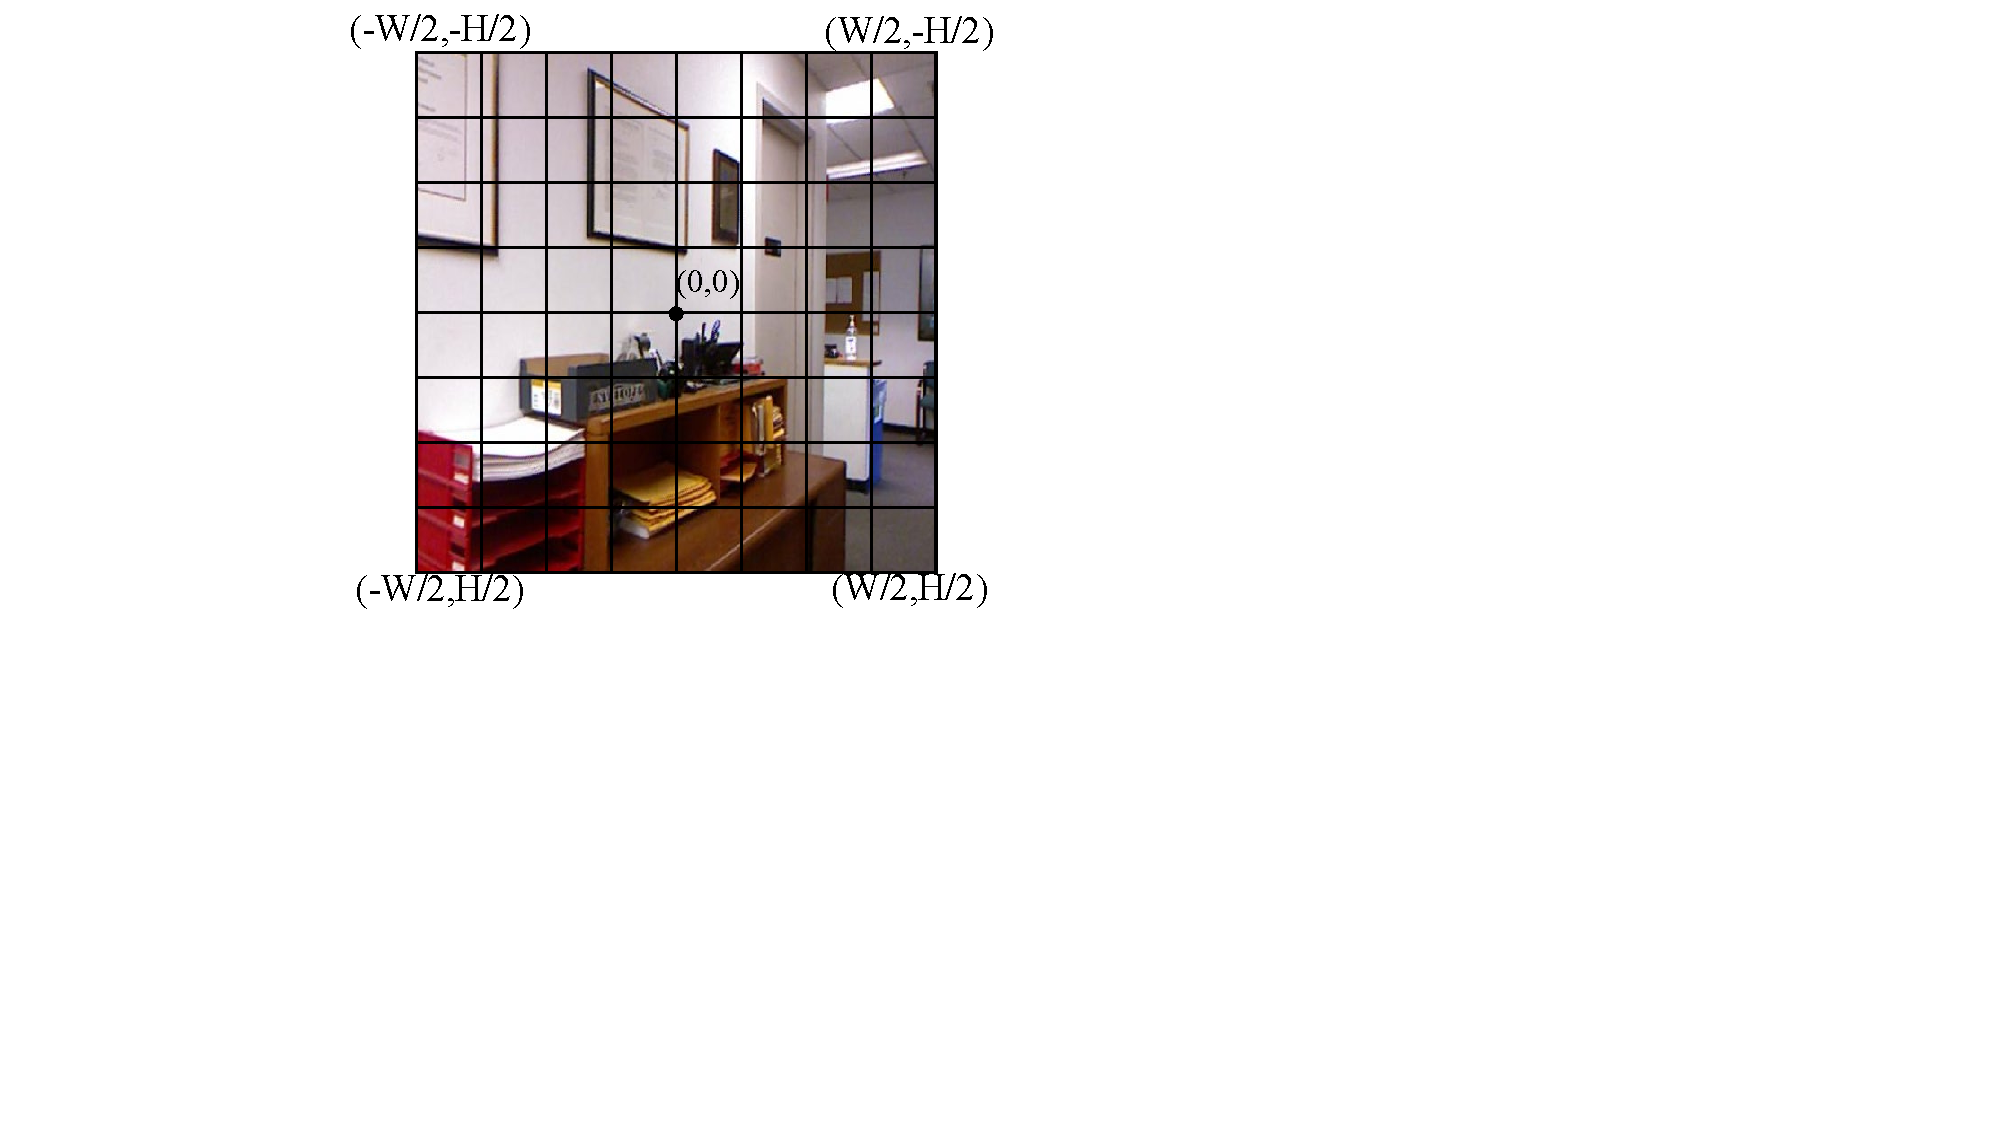
\includegraphics[width=0.4\textwidth]{imgs/coordinate.pdf}
	\caption{The coordinate grid of the benign image.}
	\label[]{coordinate}
\end{figure}

After that, 
we exploit affine transform to perform the translation.
In particular, we organize a $2 \times 3$ matrix 
$\mathbf{A}_\theta$ to translate the patch on 
the benign image:
\begin{align}
	\left[
		\begin{array}{ccc}
			1 & 0 & t_x \\
			0 & 1 & t_y \\
		\end{array}
		\right]      
\end{align}
where $t_x, t_y$ denote the offsets in 
horizontal and vertical directions, respectively. 
Denote the $[t_x,t_y]^\top$ as $\mathcal{T}$.
Initial values of $\mathcal{T}$ is $[0,0]^\top$, 
which represents that the patch locates on the center of the image.
The homogeneous coordinate of the patch is noted as $G$.
Given an affine transform matrix, we can obtain a new 
coordinate$G'$ from $G$:
\begin{align}
	{G'}^T = A_{\theta}~{G}^T
\end{align}
Denote the coordinate of each pixel of the patch 
as $G_i = (x_i, y_i, 1)$,
they are moved to a new coordinate:
\begin{align}
	\label[]{new coordinate}
\begin{pmatrix}
	x_t\\
	y_t	
	\end{pmatrix} = 
		\left[
			\begin{array}{ccc}
				1 & 0 & t_x \\
				0 & 1 & t_y \\
			\end{array}
			\right] 
			\begin{pmatrix}
				x_s\\
				y_s\\
				1	
				\end{pmatrix} 
\end{align}
Based on this, the patch $\delta$ can perform 
arbitrary translation on the benign image.

\subsubsection{Objective Function}
\label[]{Objective Function}
As illustrated before, our patch slides on the image through
affine transform in an optimization manner.
During optimization, we consider two factors: 
destructiveness and inconspicuousness.
Based on this considerations, 
we design two objective objectives.
%and what appearance of the patches are more 
%inconspicuous.
%The last consideration about the appearance is addressed
%by perspective geometry, 

\paragraph{Destructiveness}
The MDE model $f_{mde}$ generates depth maps, 
whose pixel values represent the distance from the sampled 
scene to the sensor.
We aim to obtain the adversarial examples that have
strong destructiveness,
that is, 
to maximize the error between depth maps predicted form
adversarial examples and ground truth depth maps.
We design $\mathcal{L}_{vulnerable}$ to search for the 
vulnerable location: 
\begin{align}
\mathcal{L}_{vulnerable} = \Vert f_{mde}(I^{adv}) - D^{*} \Vert_{p}
\end{align}
where $P$ represents a distance metric, 
we use $L_1, L_2$ and Huber distance in our experiments.

\paragraph{Inconspicuousness}
For better inconspicuousness, we disguise the patch 
as a graffiti, which can be usually found on 
blank walls or furnitures. 
We design $\mathcal{L}_{blank}$ to help the patch to 
find blank areas, 
$\mathcal{L}_{blank}$ consists of two optimization sub-terms:
\begin{align}
	\label[]{blank}
	\mathcal{L}_{blank} = \mathcal{L}_{smooth}+\mathcal{L}_{white}
\end{align}

In Eq.~\ref{blank}, $\mathcal{L}_{smooth}$ constrain the patch locate
on areas that have low texture complexity:
	\begin{align}
		\label[]{smooth}
		\mathcal{L}_{smooth} = 
		-\frac{\sqrt{\partial_x^2 (I-m \odot I) + \partial_y^2 (I-m \odot I)}}{n} 
 	\end{align}
where $\partial_x$ and $\partial_y$
denote the gradient in $x$ and $y$ directions, respectively,
and $n$ is the number of valid pixels in the mask $m$.
Because our patch is composed by black lines, 
which means they are more likely to appear in white areas.
So we design the $\mathcal{L}_{white}$ to constrain the patch locate
on white areas:
	\begin{align}
		\label[]{white}
		\mathcal{L}_{white} = \frac{\sum_{1}^{n} m \odot I}{n} 
 	\end{align}

The $\mathcal{L}_{vulnerable}$ and $\mathcal{L}_{blank}$ 
are summed up in a linear manner 
to compose our final objective function:
\begin{equation}
\begin{aligned}
	&\mathcal{L}_{total} = \mathcal{L}_{vulnerable} +
	\mathcal{L}_{blank}\\ 
\end{aligned}
\end{equation}

\subsubsection{Location Optimization}
As indicated in Eq.\ref{new coordinate},
the target coordinates of the patch $G'_i$ 
are continuous values. 
In other words, 
the value of the target pixels are computed by a sampling method. 
We adopt bilinear interpolation sampling to determine the value of 
the target pixel. 
%which is proved to be differentiable in 
%\textit{spatial transformer networks}~\cite{stn}.
By maximizing the $\mathcal{L}_{total}$, 
we can optimize the offsets $\mathcal{T}$ step by step.
\begin{align}
    \mathcal{T}_0 = [0,0]^\top, 
	\mathcal{T}_{s+1} = Clip\{\mathcal{T}_{s} + 
	\alpha{\bigtriangledown_{\mathcal{T}}\mathcal{L}_{total}}\}. 
	\label[]{optimization}
\end{align}
where $\mathcal{T}$ denotes the translation vector $[t_x,t_y]^\top$.

The whole process is proved to be differentiable:

To avoid patches overflowing from clean images, $t_x$ and $t_y$
are clipped between $(\frac{W-w}{W},-\frac{W-w}{W})$ and
$(\frac{H-h}{H},-\frac{H-h}{H})$, respectively.
In our experiments, the size of clean images is $224 \times 224$
and the size of the patch is $28 \times 28$, which means
the $t_x$ and $t_y$ are both clipped between $(0.875,-0.875)$.
For all experiments we set 
$\alpha = 0.004$, 
total optimization step is 50 steps.

\subsection{Appearance Altering}
\label[]{Appearance Altering}
In location searching phase, our method find a sensitive
and concealed location for the patch.
At this phase, we alter the appearance of the patch 
according to the perspective transformation principle 
to make it looks more natural.
The phase can be seen in Fig.~\ref{stream}(b).

\begin{figure}[tb]
	\centering
	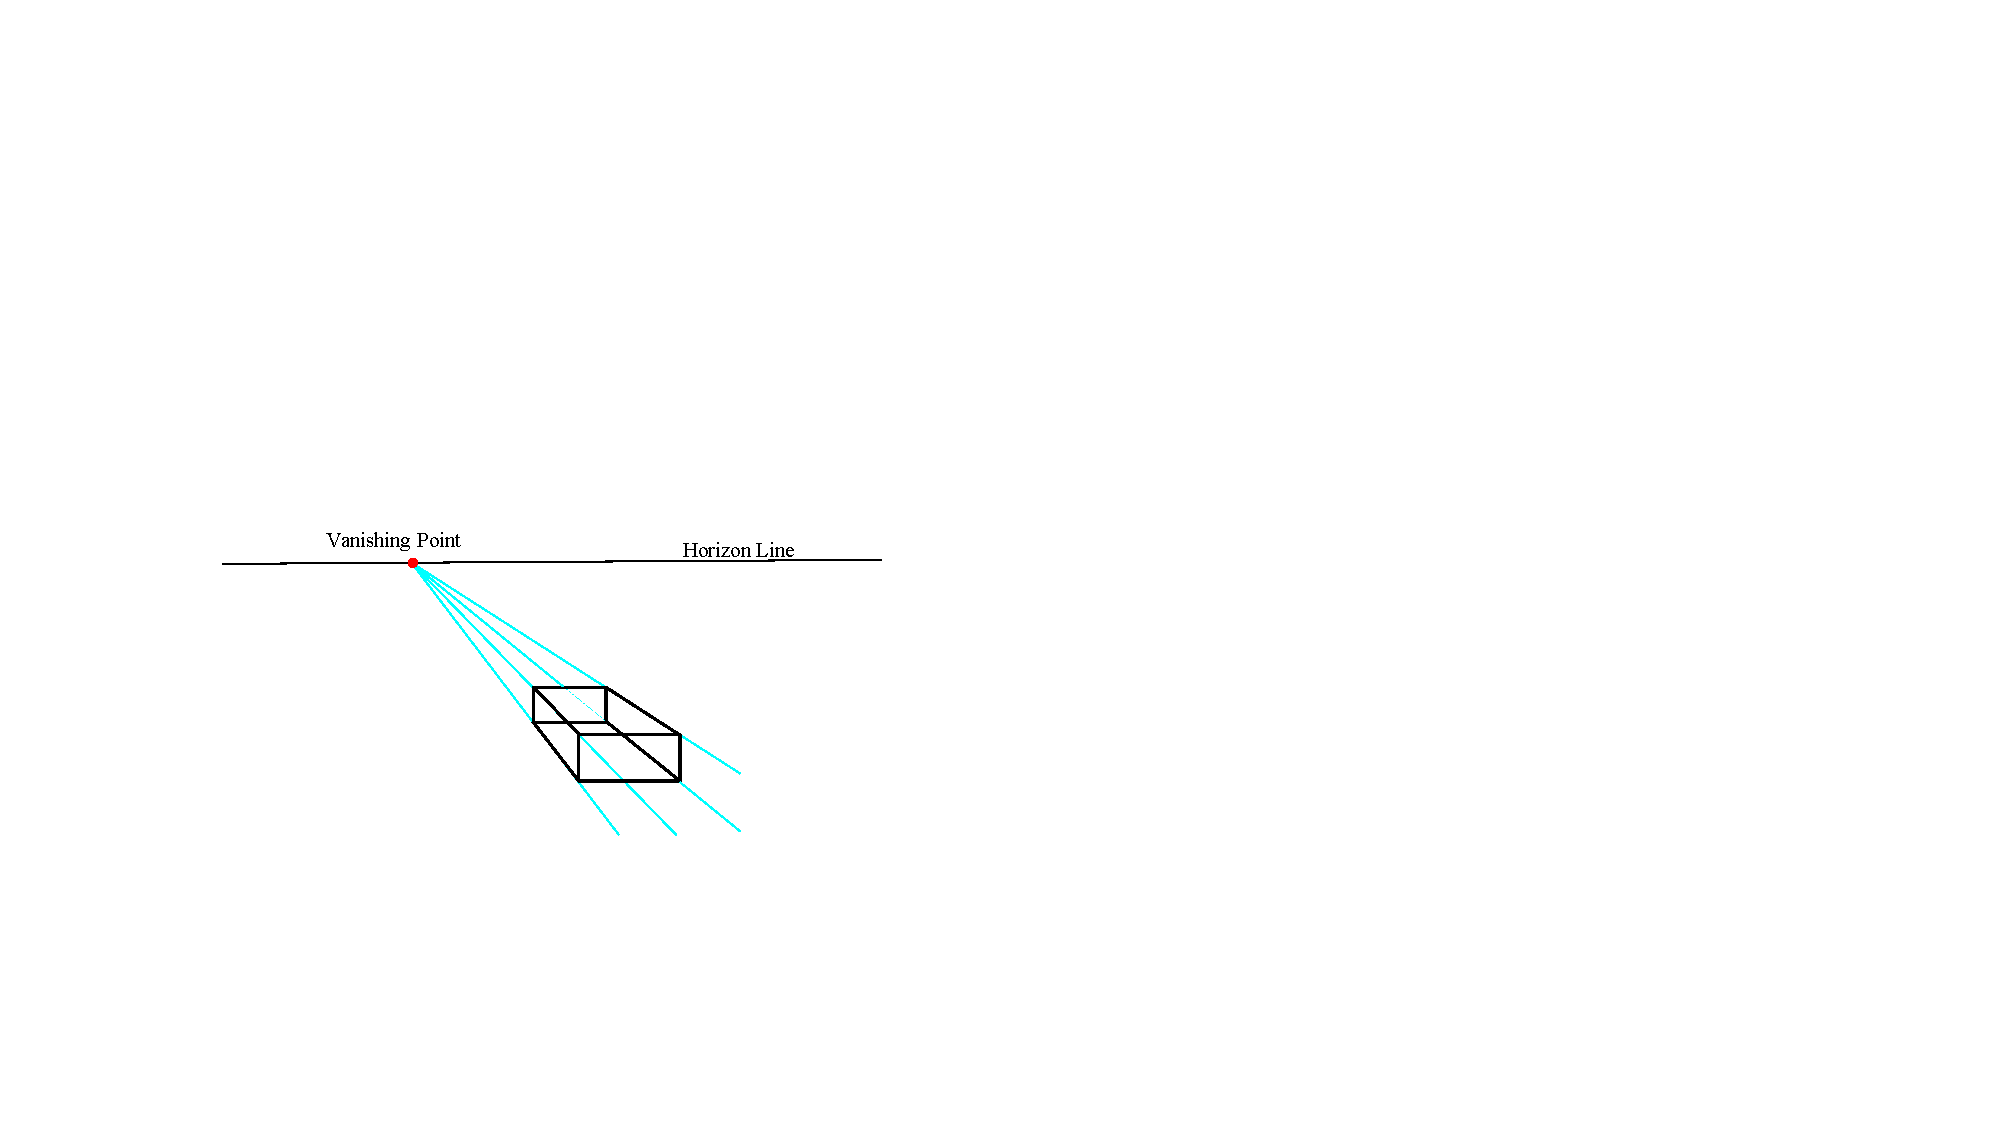
\includegraphics[width=1\linewidth]{imgs/perspective.pdf}	
	\caption{Diagram of single point perspective drawing:
	All the vanishing lines lead to the vanishing point.
	The horizontal and vertical lines, however, 
	remain parallel to each other.}
	\label[]{perspective}
\end{figure}
For better visualization quality, we follow
the principle of perspective drawing: 
the vanishing point is where all parallel lines 
intersect and is always on the horizon line.
Fig~\ref{perspective} clearly 
illustrates this principle.

To obtain the vanishing point, we detect straight 
lines in the adversarial examples
with \textit{Hough} transform and extend them.
The intersection of these lines is vanishing point
obviously.

As illustrated in Fig~\ref{stream}(b), 
if we connect the left-top point and 
vanishing point, the right-top point should lay on this 
line. Same with the bottom line. 
Base on this principle, we calculate four corrected
corner coordinates. The perspective
transforms in this phase are implemented with 
\textit{OpenCV}. 

\section{Experiments}
\label[]{Experiments}
\begin{figure*}[h]
	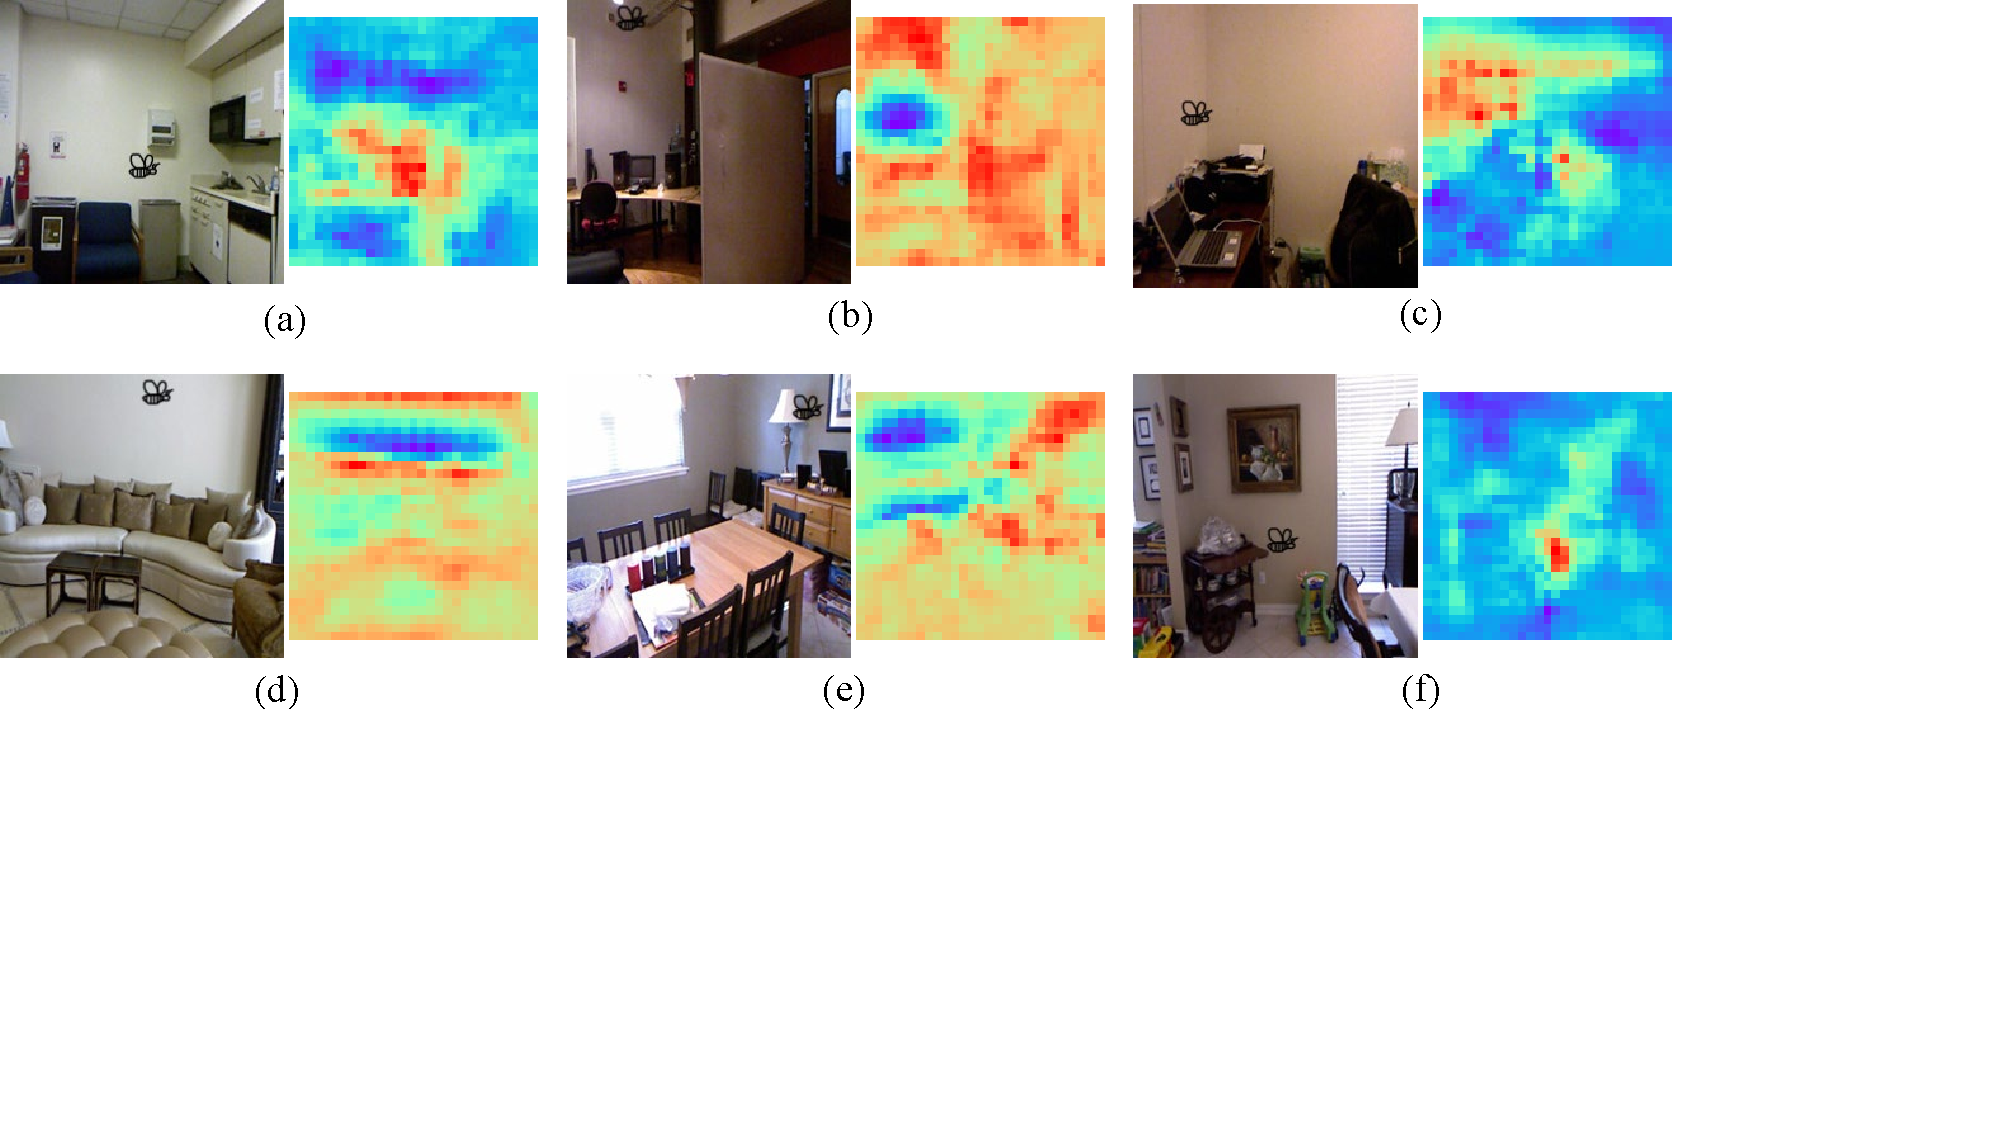
\includegraphics[width=1\textwidth]{imgs/patch_on_scenes.pdf}
	\caption{The final attack locations searched by our method (left) 
	and corresponding MAE maps (right). 
	Then calculate MAE maps, the offsets of the patch 
	are clamped between -0.875 and 0.875, 
	which makes the maps a little smaller than the RGB images.
	}
	\label[]{patch_on_scenes}
\end{figure*}
In this section, we conduct several experiments to exhibit 
the results of our automatic and inconspicuous attack
method on a MDE model. 
%As mentioned before, we consider three factors: attack effect, 
%which area of the adversarial example is more inconspicuous 
%and how to make the patches more inconspicuous. 
The implemention detail including datasets, data pre-processing 
and experiment environment is introduced in
Sec.~\ref{Implemention Detail}.
Then we demonstrate the automatic optimization performance 
in Sec.~\ref{Automatic Searching}. 
Finally, our attack effects are shown by visualization
and quantitative comparison
in Sec.~\ref{Visualization Attack Results} and 
Sec.~\ref{Quantitative Attack Results}. 

\begin{figure*}[h]
	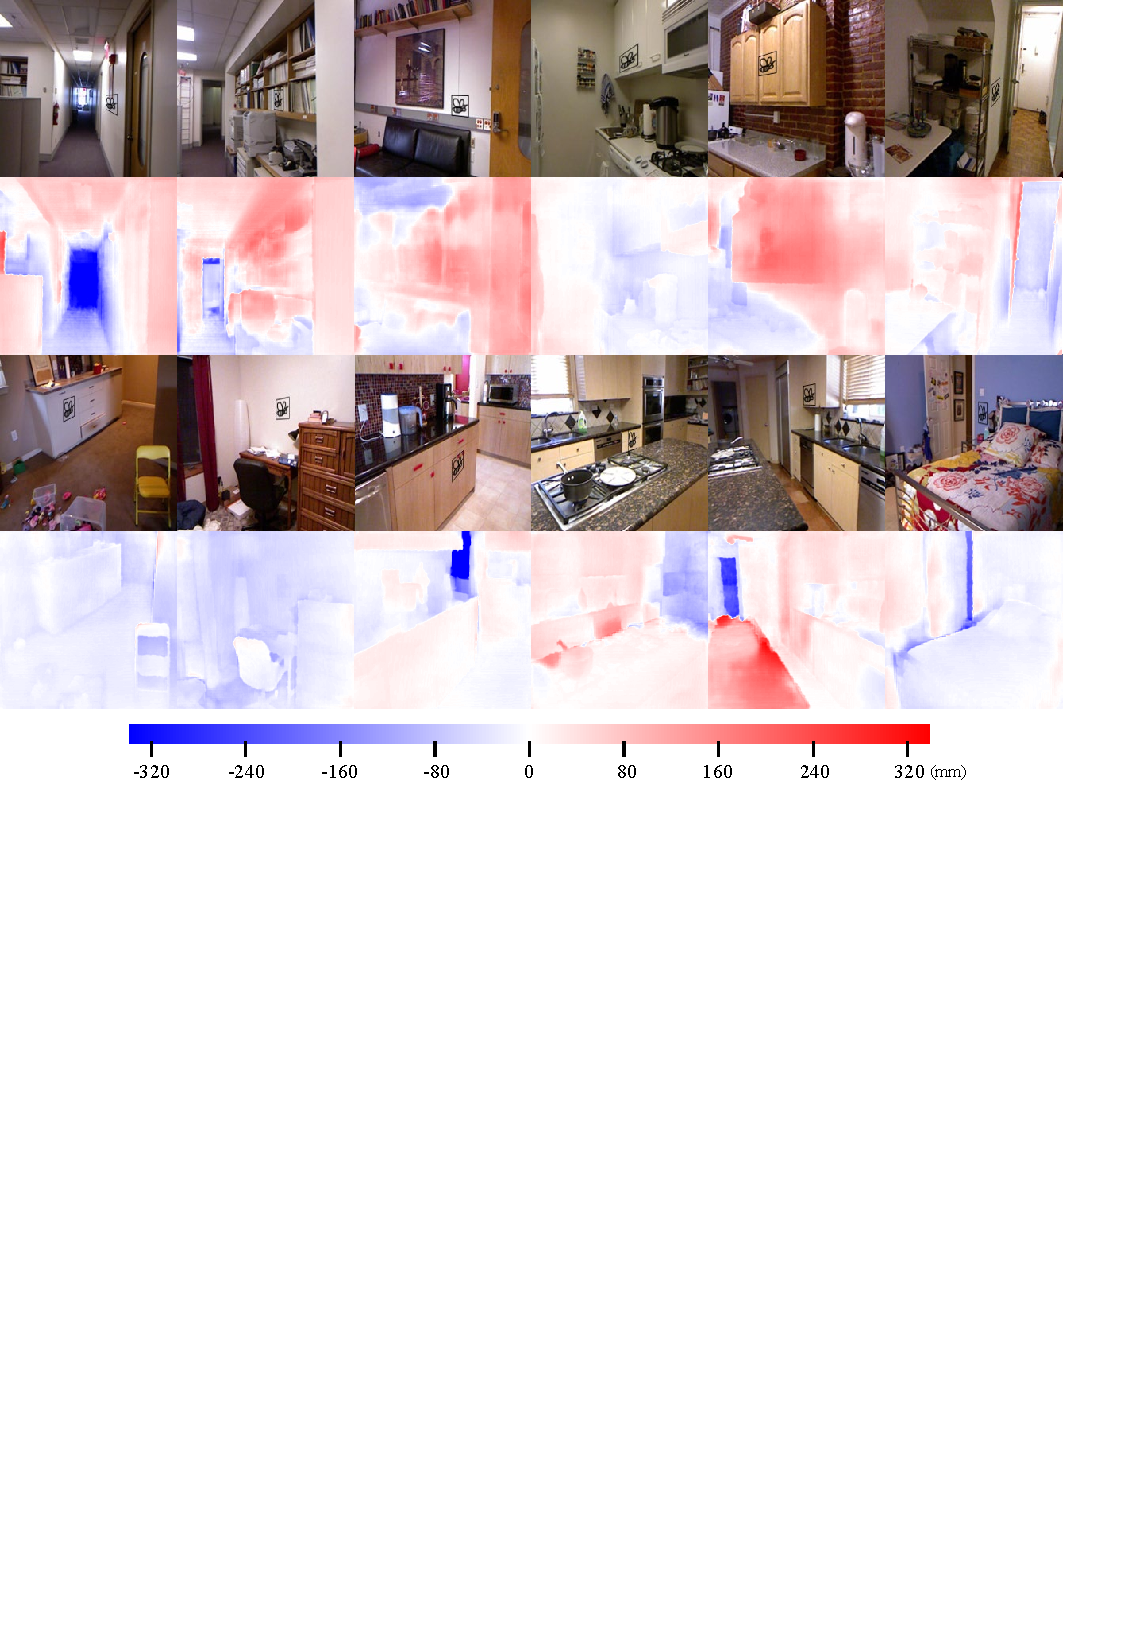
\includegraphics[width=1\textwidth]{imgs/results.pdf}
	\caption{The visualization of our patch attack
	method. The first and third rows are $I^{adv}$.
	The second and fourth rows are the visualization
	of prediction error: 
	$f_{mde}(I^{adv}) - D^{*}$.
	The color bar down the results explicates the 
	error value intuitively.
	We emphasize the patches using surrounding 
	black boxes, which are transformed in the 
	altering appearance phase also.}
	\label[]{results}
\end{figure*}
\subsection{Implemention Detail}
\label[]{Implemention Detail}
To study the effect of our patch adversarial examples,
we examine the robustness of a supervised method 
Fastdepth~\cite{Wofk_2019_ICRA}. 
The examined MDE model is trained and evaluated on NYU depth v2
~\cite{Silberman_2012_ECCV}, 
a widely used indoor dataset with 0-10 meters depth range.
NYU depth v2 consists of 1449 densely annotated depth and 
RGB images pairs,
according to Eigen~\textit{et al}~\cite{Eigen_2014_nips},
795 of them are split to train dataset and the rest are
split to test dataset.
For the image pre-processing, we followed the process in
Fastdepth: images are resize to $250 \times 333$ firstly, 
secondly, center cropped to $224 \times 304$, in the end 
they are resized to $224 \times 224$.
As mentioned in~\ref{Patch Design}, adversarial examples 
generated with simple line-drawn patches looks more natural.
Therefore, we select a size of 28×28 bee drawing from 
QuickDraw~\cite{quickdraw} to generate
our adversarial examples.

We focus on four metrics used in previous works to evaluate 
the attack effect: 
\begin{align}
 RMSE=\sqrt{\frac{1}{\lvert N \rvert} \sum\nolimits_{i\in N}\lvert|D_i - D_i^*\rvert|^2} 
\end{align}

\begin{align}
 MAE=\frac{1}{\lvert N \rvert} \sum\nolimits_{i\in N}|D_i - D_i^*| 
\end{align}

\begin{align}
  Abs \ Rel=\frac{1}{\lvert N \rvert}\sum\nolimits_{i \in N}\frac{\lvert D_i - D_i^* \rvert}{D_i^*}
\end{align}

\begin{align}
  Threshold: \% \ of \ D_i \ s.t. \max(\frac{D_i}{D_i^*},\frac{D_i^*}{D_i})=\delta < thr 
\end{align}
where $D_i$ represents the predicted depth map from $I^{adv}$, 
$N$ is the pixel number of $I^{adv}$, and $thr$ denotes three 
threshold $1.25$, $1.25^2$, $1.25^3$. 
Besides the accuracy, we also record our runtime, which
can show the efficiency of our attack method.

\begin{table*}
    \centering  % 显示位置为中间
    \caption{Accuracy of our method, best results are boldfaced}  % 表格标题
    \label[]{comparison table}  % 用于索引表格的标签
    %字母的个数对应列数,|代表分割线
    % l代表左对齐,c代表居中,r代表右对齐
    \begin{tabular}{c|c|c|c|c|c|c|c|c}  
		\toprule
      \multicolumn{2}{c|}{}&RMSE &MAE
	  &Absrel &$\delta_1<1.25$ 
	  &$\delta_2<1.25^2$&$\delta_3<1.25^3$&Runtime \\  % 表格中的内容,用&分开,\\表示下一行
      \midrule
      %& & & \\[-6pt]  %可以避免文字偏上 
      \multicolumn{2}{c|}{fastdepth (baseline)}&0.600&0.427&0.162&0.771&0.927&0.988&- \\
      \hline  % 表格的横线
      \multirow{3}{*}{Ours}&$L_1$&0.643&0.464&0.175&0.738&0.920&0.973&0.772  \\
      					&$L_2$&0.641&0.461&\textbf{0.177/9.3\%}&0.739&0.921&0.973&0.781  \\
      	&Huber&\textbf{0.648/6\%}&\textbf{0.466/9.1\%}&0.176&\textbf{0.737}&\textbf{0.919}&\textbf{0.972}&0.772  \\
		\bottomrule
    \end{tabular}
  \end{table*}
\subsection{Automatic Searching} 
\label[]{Automatic Searching}

Given an clean image, 
our attack method can search the sensitive area and stick
the patch on this area. To better demonstrate our search effect, 
we calculate the MAE 
maps of test images. The MAE maps are obtained using
following step: beginning from the left top corner, 
we use strides 7 to slide the patch 
step by step and calculate 
the MAE of each position.
The red and violet color in the maps represent 
higher and lower 
MAE values, respectively.
As you can see from Fig~\ref{patch_on_scenes}, 
our method can accurately search the sensitive area of the image.
Note that to emphasize our search effect, we didn't use the 
$\mathcal{L}_{blank}$~Eq.\ref{blank}
in this experiment. 

\subsection{Visualization Attack Results} 
\label[]{Visualization Attack Results}
For inconspicuousness, we show the adversarial examples
in the first and third rows. The black box shows that
our adversarial examples follow the principle 
of perspective drawing. Besides the patches lay on 
walls and furniture, which makes our examples look like 
graffiti and more harmonious in indoor scenes.

For destructiveness, we show the 
prediction error in the sencond and fourth row.
Our method achieves $320mm$ max error. Prediction results
from $I^{adv}$ are usually nearer than ground truth 
depth maps in far-range areas, for instance, 
the blue areas in Fig~\ref{results}.
However, the results are farther in near-range areas,
which means our adversarial examples mislead the MDE 
system and make the prediction results converge to 
middle distances.

\subsection{Quantitative Attack Results} 
\label[]{Quantitative Attack Results}

We show our attack effect by quantitative comparison in 
Table~\ref{comparison table}. To the best our knowldege,
we are the first to attack MDE systems using patches.
There does not exist much related works.
So we compare the baseline MDE method, fastdepth between
our method with different $\mathcal{L}_{attack}$.
We degrade the MAE by 9.13\%, as a contrast, 
Wong~\cite{Wong_2020_NIPS} achieve 10\% accuracy loss
(closer or farther)
on each pixel of the depth.
However, they rely on the guidance of the modified ground
truth depth maps, in other words, they modify the ground
truth depth value down or up 10\% in each pixel, 
and use the modified
maps as supervision. Besides, they use elaborately designed
perturbations to generate adversarial examples.

%We visualize the serach path in Fig~\ref{search_path}.
%\begin{figure*}
%	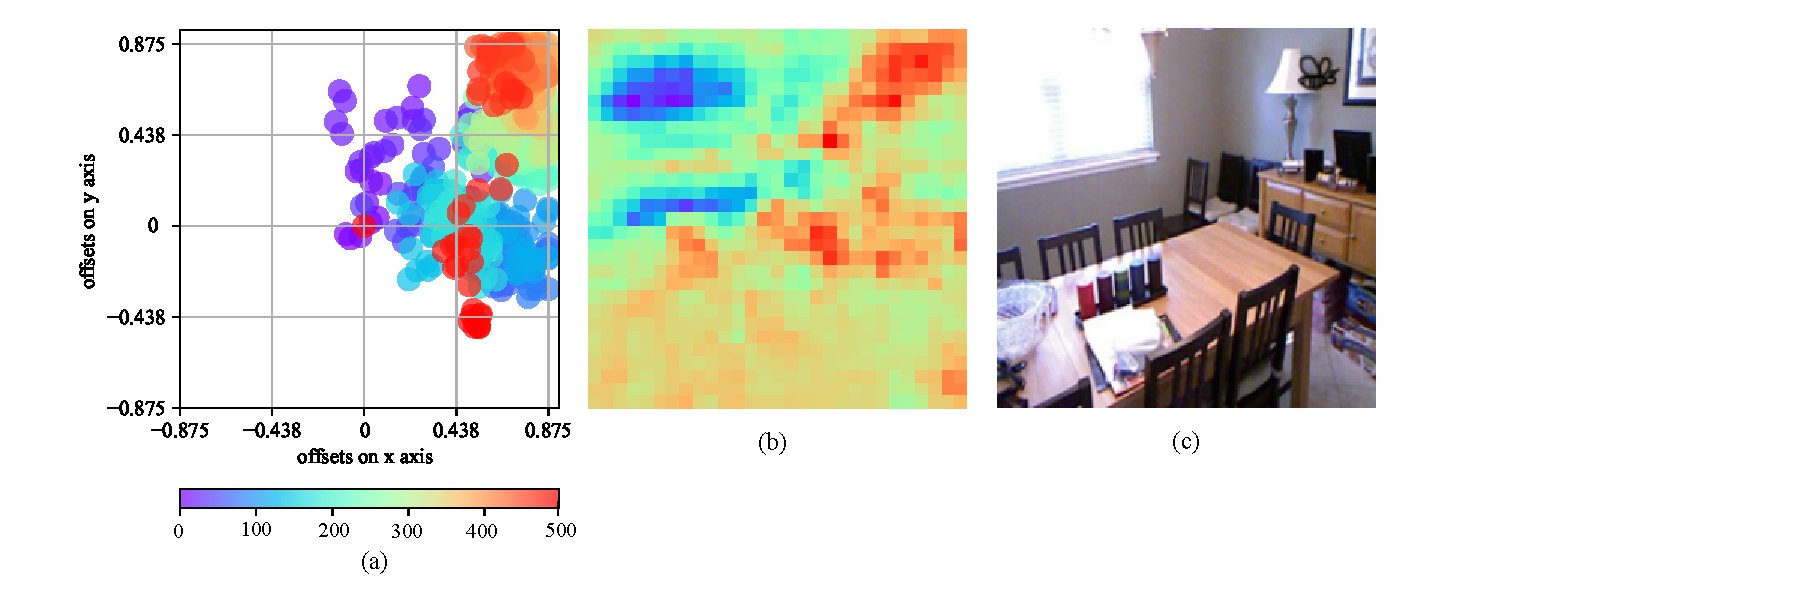
\includegraphics[width=1\linewidth]{imgs/search_path.pdf}
%	\caption{The search path of~\ref{patch_on_scenes} (e), the
%	color from violet to red represent the search steps from 0
%	to 500.}
%	\label[]{search_path}
%\end{figure*}

%We use different stickers to calculate their MAE maps on the 
%same image, to investigate the impact of different patches on 
%the sensitive area's location in the image. As shown 
%in Fig~\ref{patches_on_one_scene}, the distribution of sensitive 
%and robust areas in (c)~(f) is similar, the sensitive areas
%are concentrated in the center, among them
%(d) and (f) almost looked the same. However there are 
%some differences between (h),(g) and (c)~(f). Intuitively, 
%this is caused by the variations of patch\ding{176} and 
%\ding{177} in saptial structure. Based on this, 
%we conclude that, to similar patches, the distribution 
%of an image's sensitive and robust area is usually the same. 
%The similarity is more significant along with the smaller size. 
%
%\begin{figure*}
%	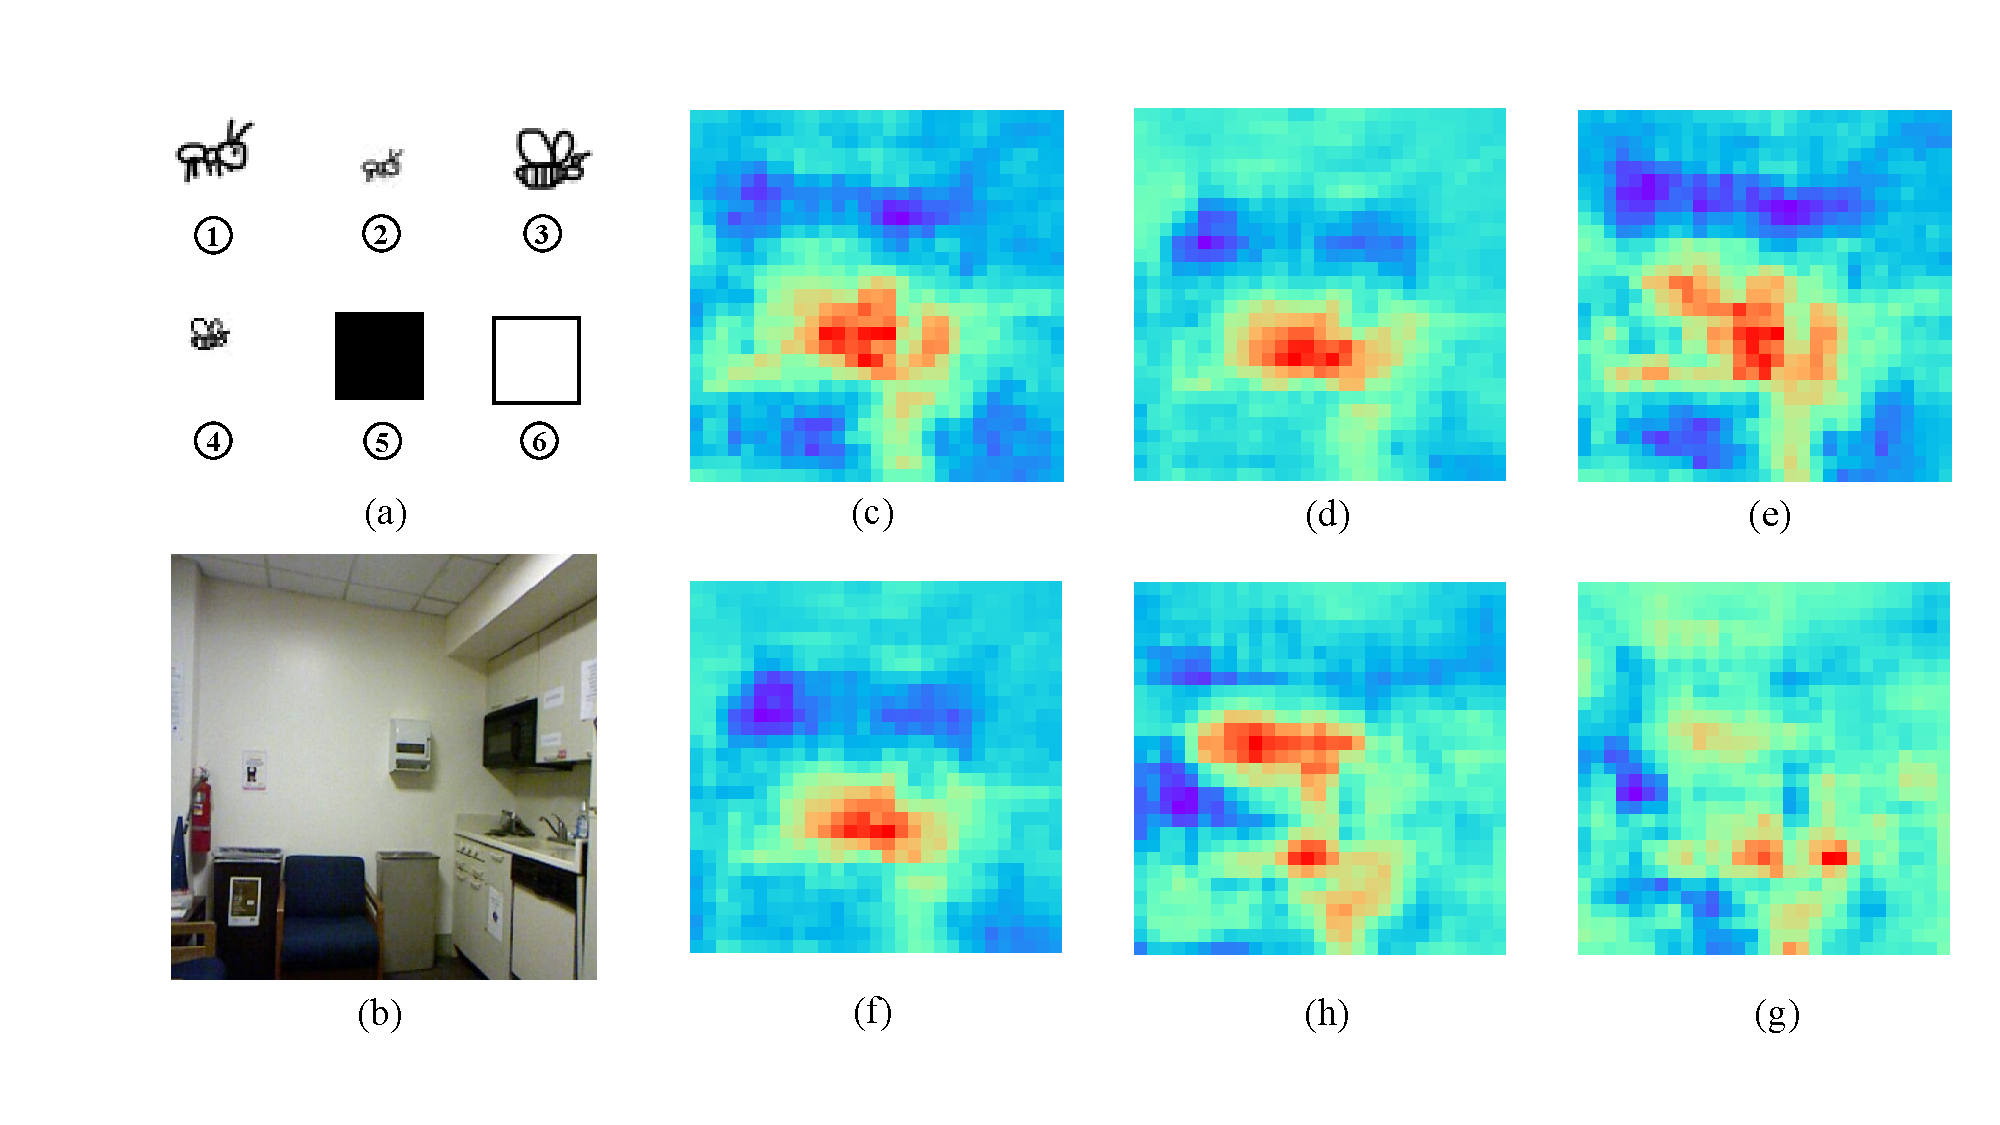
\includegraphics[width=1\linewidth]{imgs/patches_on_one_scene.pdf}
%	\caption{There are 6 different
%	patches in (a), they are stuck in (b) to 
%	calculate MAE maps (c~g). The placement of (c~g) is the same 
%	as the patches' placement in (a). Patch \ding{173} and \ding{175}
%	are down sampled from \ding{172} and \ding{174} with factor 0.5.
%	Patch \ding{176} is a black patch filled with 0 and patch 
%	\ding{177} is a white patch filled with 1.
%	The black box is for visualization this white patch.}
%		
%	\label[]{patches_on_one_scene}
%\end{figure*}

\section{Conclusion}
\label[]{Conclusion}
We attacked an MDE system using our fast, 
physical-realizable, automatic and inconspicuous 
patch attack method. Fast because it doesn't lean 
on any generative networks. Physical-realizable 
because the effect can be simulated by sticking a 
real patch on the sensitive spot. Automatic 
because it is optimized by gradient descent. 
Inconspicuous because our method conceals the patch 
as graffiti. Our experiments showed that the depth 
maps predicted by the target MDE system lost some accuracy. 
Our work revealed the probability that an accident 
could happen due to drawing graffiti intentionally 
or unintentionally. Future works 
should pay more attention to multimodal fusion 
or provide robust constraints for MDE networks.

\section{Acknowledgements}
xxx

%%%%%%%%% REFERENCES
{\small
\bibliographystyle{ieee_fullname}
\bibliography{egbib}
}

\end{document}
